 \documentclass{article}
\usepackage{tikz}
\usetikzlibrary{shapes, arrows}

\tikzstyle{startstop} = [rectangle, rounded corners, minimum width=3cm, minimum height=1cm, text centered, draw=green, fill=red!30!yellow]
\tikzstyle{arrow} = [thick, ->, >=stealth]
\begin{document}

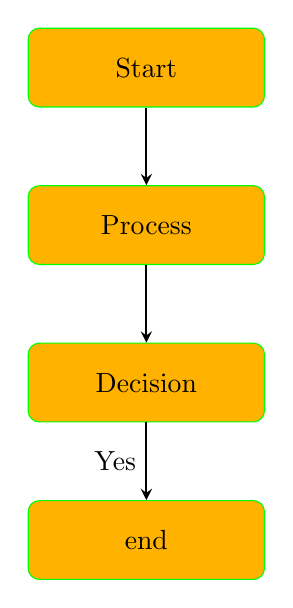
\begin{tikzpicture}[node distance=2cm]
\node(start) [startstop] {Start};
\node(process) [startstop, below of=start] {Process};
\node(decision) [startstop, below of=process] {Decision};
\node(end)[startstop, below of=decision] {end};
\draw [arrow] (start) -- (process);
\draw[arrow] (process) -- (decision);
\draw[arrow] (decision) -- node[anchor=east] {Yes} (end);
\end{tikzpicture}
\end{document}
